\usecasebase{Visualizzazione lista delle prenotazioni}
\label{usecase:Visualizzazione lista delle prenotazioni}

\begin{figure}[h]
	\centering
	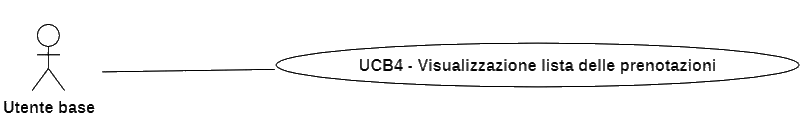
\includegraphics[width=0.8\textwidth]{./uml/UCB4.png} 
	\caption{Visualizzazione lista delle prenotazioni}
	\label{fig:UCB4}
  \end{figure}

\begin{itemize}
	\item \textbf{Attore principale:} Utente base.

	\item \textbf{Precondizioni:}
	      \begin{itemize}
		      \item L'Utente ha eseguito correttamente l'accesso al Sistema come Utente base (vedi \autoref{usecase:Effettua accesso}).
		      \item L'Utente base ha precedentemente effettuato una prenotazione (vedi \autoref{usecase:Prenotazione di un tavolo}).
	      \end{itemize}


	\item \textbf{Postcondizione:}
	      L'Utente base visualizza la lista di tutte le sue prenotazioni.

	\item \textbf{Scenario principale:}
	      \begin{enumerate}
		      \item L'Utente base visualizza la lista delle prenotazioni che ha effettuato;
		      \item Il Sistema mostra, di \textit{default}, la lista delle prenotazioni categorizzate nei seguenti stati:
		            \begin{itemize}
			            \item In attesa.
			            \item Accettata.
			            \item Rifiutata.
			            \item In corso.
			            \item Terminata.
			            \item Annullata.
		            \end{itemize}
		      \item Il Sistema mostra la lista in tale ordine basato sugli stati.
	      \end{enumerate}
\end{itemize}